\chapter{基于深度学习方法的无人机目标跟踪方法研究}
\label{chap:main}


\section{引言}
针对目标检测问题,很多学者提出了不同的解决方法,但目标实时监测问题中的所涉及的目标尺度变化、被遮挡和实时性等问题仍然没有得到有效解决。本章针对无人机自主降落过程中的目标跟踪问题进行进一步分析,并提出了满足实时性需求的目标跟踪算法。

\section{基于ImageNet神经网络设计方法}
传统的跟踪方法的主要工作是在线跟踪,算法在运行过程中,基本不涉及离线计算。这些跟踪算子(Tracker)主要通过数学公式来完成对跟踪目标特征的描述,这种描述能力的好坏决定着这个算法性能的优劣。同时,由于传统方法的跟踪算子无法重复利用大量现有数据,其算法性能无法随着数据量的增加而得到持续性改善。这种方法适用于典型目标的跟踪,例如行人跟踪和人脸跟踪等[6, 30]。
随着计算机运算能力的增强以及大量人工标记的数据库规模增大,基于深度神经网络方法的跟踪算法得到了进一步发展。
一种方法是在线训练在线更新算法。这类算法在训练过程中,利用海量数据信息,对网络进行大规模训练训练。在跟踪过程中,网络初始参数基于预训练网络,并根据在线数据对参数进行进一步调整。[70 71 72]。这类方法的跟踪速率大概在0.8 fps 到4 fps之间,不能满足一般的实时性系统需求。

\begin{figure}[htb]   
	\centering
	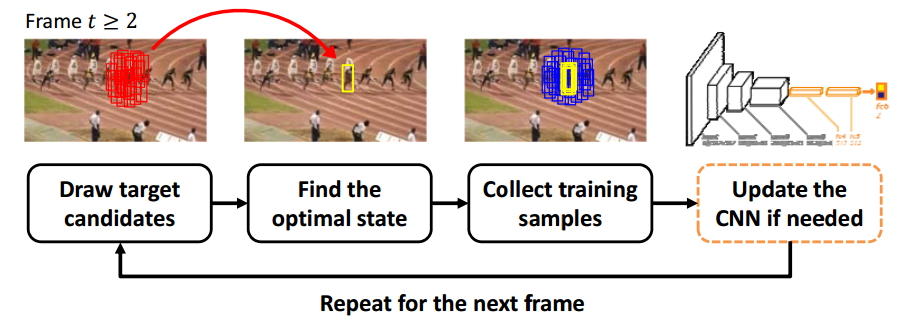
\includegraphics[width=\textwidth]{figs/chp03/chp03_01_CNN_One_Shot_Process.pdf}
	\caption{CNN方法处理One-shot Tracking问题基本框架}
	\label{fig:161002.chp03_01_CNN_One_Shot_Process}
\end{figure}

另一种方法是离线训练在线不更新算法。这类算法所利用的数据量更大和训练时间更长,训练之后稳定下来的网络参数在后续的测试过程中不发生变化。
Generic Object Tracking Using Regression Networks(GOTURN)网络是一种离线网络。这种网络主要通过离线训练得到节点权重,在后续的跟踪过程中不需要进行在线训练,实时性好,在使用GPU加速的情况下,跟踪帧频可以到达100Hz。
这是一种End-to-end的训练。在训练的输入数据中,只需要知道原始图像和目标区域,并不需要目标的类别等更高级别语义信息。在输出数据方面,该方法直接给出目标的具体位置。

\subsection{GOTURN网络的实现}



\subsection{搜索区域迭代方法}
因为神经网络方法的通用性,网络结构输出的搜索区域一般是置信度最高的区域,

如上图所示,红色矩形框:系统识别到的目标。
绿色矩形框:真实参考值。
目的:希望通过对红色矩形的微调,即Bounding Box Regression,更接近绿色矩形。
矩形框的表达一般用四维变量$(x, y, w, h)$表示,即矩形框中心的像素位置以及矩形框的宽度和高度。

\begin{figure}[htb]   
	\centering
	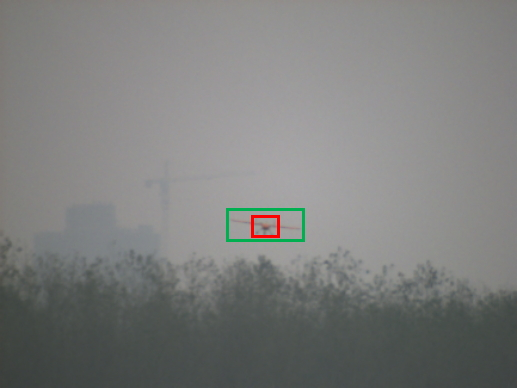
\includegraphics[width=\textwidth]{figs/chp03/chp03_02_bbox_regression.pdf}
	\caption{目标识别区域和真实值之间的差异}
	\label{fig:chp03_02_bbox_regression}
\end{figure}


迭代方法
- 寻找一种映射 $f$,使得$f(x_P, y_P, w_P, h_p) = (x_{\hat{G}}, y_{\hat{G}}, w_{\hat{G}}, h_{\hat{G}})$,其中$(x_{\hat{G}}, y_{\hat{G}}, w_{\hat{G}}, h_{\hat{G}}) \approx (x_G, y_G, w_G, h_G)$

- 定义目标区域(Proposal Region) $P=(x_P, y_P, w_P, h_p)$, 真实值区域(Ground-truth Region) $G = (x_G, y_G, w_G, h_G)$,预测区域 $\hat{G}=(x_{\hat{G}}, y_{\hat{G}}, w_{\hat{G}}, h_{\hat{G}})$

- 先平移$(\Delta_x, \Delta_y)$
$$x_{\hat{G}} = w_{P}d_x(P)+x_P$$
$$y_{\hat{G}} = h_{P}d_y(P)+y_P$$

- 再尺度变化$(S_w, S_h)$
$$w_{\hat{G}}=w_{P}exp(d_w(P))$$
$$h_{\hat{G}}=h_{P}exp(d_h(P)$$

- Regression过程

- 输入:$P=(x_P, y_P, w_P, h_p)$这个区域的CNN图像特征,而不是简单的四个点,训练阶段还包括真实值 $T=(x_T, y_T, w_T, h_T)$

- 输出:四个尺度变换$d(P)=(d_x(P), d_y(P), d_w(P), d_h(P))$

$$d_x(P)=(x_{\hat{G}}-x_P)/w_P$$
$$d_y(P)=(y_{\hat{G}}-y_P)/h_P$$
$$d_w(P)=log(w_{\hat{G}}/w_P)$$
$$d_h(P)=log(h_{\hat{G}}/h_P)$$

- 四个基本信息的线性组合方程 $\Phi(P)$

- 在$P$情况下的预测值 $d(P)=\omega^T\Phi(P)$

- 损失函数(可以有很多种)
$$Loss=\sum^N_i(T^{(i)}-\omega^T\Phi(P^{(i)}))^2$$
$$L_{loc}(P,T) = \sum_{i}^N\text{smooth}_{L_1}(T^{(i)}-P^{(i)})$$
$$\text{smooth}_{L_1}(x) = \left \{ \begin{aligned} &0.5x^2 & |x| \le 1\\ &|x|-0.5 & \text{otherwise}\end{aligned} \right.$$
​

- 目标函数
$$\omega^*=\mathop{\arg\min}_{w}\sum^N_i(T^{(i)}-\omega^T\Phi(P^{(i)}))^2+\lambda||\omega||^2$$



\section{基于Siamese神经网络设计方法}

\section{针对图像尺度变换的设计}
在近距离目标跟踪过程中,目标主要发生尺度方面的变化。卷积运算具有平移不变的特性,即


 